\section[第4章\q 先付钱给自已]{第4章\\ 先付钱给自已}
\label{sec:ch4}

周三早上，柔伊比前一天更早去了咖啡厅。她发现亨利站在后方，面对照片，陷入沉思中。她回想第一天遇见时，也正是这个时间点。“不好意思。”她说。

亨利微微震了一下。“哇，柔伊。”他开心的招呼说：“我正在欣赏我们都喜欢的这幅照片呢！”

“对不起。”柔伊引用前天他对她说的话：“无意要吓到你。你看得太专注了。”说着，柔伊露齿而笑，亨利也回她一笑。

“好记性啊！”他说。

柔伊看了一眼海湾小村的照片，转身对着亨利说：“我有点不解……”柔伊犹豫了一下，想着该怎么说得更清楚一些。“昨天，你说，如果我买得起咖啡，就可以买得起那张照片？还有我比想像富有？”

亨利点头。

“这句话具体是什么意思？”

\subsection{七成的人，赚的钱只够付帐单}

亨利低头，把食指压在嘴唇上了一会儿，说：“让我这么问好了，如果要买得起这幅画，你需要做哪些改变？”

“坦白说，我需要一份比现在薪水更高的工作。”

“嗯哼，”亨利说：“你不介意我讨论一些私人的问题吧？”

“怎么会呢？”柔伊说：“你都提到我的墓志铭了，还能比那个更私人吗？”

“这个想法不错。”亨利微笑：“你在哪里高就？你提过，在曼哈顿下城区？”

柔伊点头。“世贸中心一号大楼。”她简短描述了一下在旅行杂志社的工作。

“我猜，那是一份很体面的薪水。”亨利说。

“很体面。”柔伊同意地说道：“但是不体贴。住在布鲁克林区不便宜。”

“这是实话。如果可以，我想再问一句，你在这个位置上做多久了，很长时间吗？还是很短时间？”

“前后6年了。”

“很好。这个时间足够一个年轻人发挥专长，累积经验，得到提升机会。我猜想，你现在的薪水要比6年前多一点，是吗？”

“是的。”柔伊回答。

亨利也点点头。“那么，你现在比6年前富有一些了吗？”

柔伊眨一眨眼睛。“更富有一些？”她说到富有这两个字，仿佛在说外文。

“就是手上可灵活支配的现金，比较多了吗？私房钱啊？”

事实是，2年前芭芭拉提拔她从助理编辑到副总监，薪水顺势涨了好大一截。可是看似她赚得愈多，生活花费也就愈多。她的财务更加无法平衡。

“更富有？”柔伊重复道：“没有。我必须承认，我没有更富有。”

“好，其实不只你一个人如此。我看过一篇很棒的报导。那篇文章说，在美国有半数以上的人在突然需要急用时，口袋里掏不出400美元的闲钱来。有七成的人，形容他们的生计就是刚好付帐单，甚至很多人靠信用卡预支过活。”

“这是真的。”很多人与她有同样情景，倒不让柔伊意外。反过来说，这不就是她参与编辑的旅游杂志如此畅销的原因吗？不能来一趟说走就走旅行的人，至少可以在纸上随意遨游。

“现在我们进入一个真正有趣的地方了。”亨利说。“因为在回答为什么不存钱，或者做点退休规划时，大部分人的答案和你一样，‘因为薪水不多’。”亨利浅笑着：“尽管他们这么说，但是其实这并非事实。\textbf{收入增加，并不会改善他们的处境。}”

柔伊觉得脑袋轰的一下，惊醒过来似地问：“等一下？你说什么？”她觉得一定是自己听错了。“收入高没帮助？但是……可是，收入高才有帮助啊！”

亨利摇头。“不是喔！\textbf{很多人，在收入更高之后，却花了更多钱买东西}。”

“那不是……”柔伊想说，不是真的。至少，我不是这样的。

是吗？

“你有没有常看到，”咖啡师继续说：“有些电影明星，或者运动明星，突然红起来，身价也一夜暴涨，然后接下来的新闻，就是他们又破产了。”其实，柔伊一周前就看过一篇这样的报导。“多少乐透得主最后债台高筑？对这些明星和中奖者来说，收入不是问题，对吗？问题是如何留住这些钱。”

“柔伊，一个吊诡的事实是，赚得多，特别是非常之多时，未必表示更富有。为什么会这样？因为对大多数人来说，就是赚得多花得多。\textbf{收入是水，支出是船，水涨船高}。”

亨利回头望了一眼咖啡厅，又对着柔伊说。“在你赶地铁去上班之前，还有几分钟的时间吗？”

“有的。”柔伊说。她今天早上特别提早出门，就是为了来咖啡厅。在跟着亨利往小圆桌走过去时，柔伊又想起了那张照片：收入是水，支出是船。

\textbf{水太多，会翻船；水太少，会搁浅}。

“要富有，要能财务自由。”亨利走到桌边，转头对着柔伊说：“其实很简单，只要做到三步骤。”

“让我猜猜，”柔伊说：“写一首排行前40名的畅销歌曲、中乐透、有个有钱姨妈，而且她还特别爱你，把你列为继承人。”

亨利笑着站起来，柔伊在前天坐的位置上坐下来。

“我称之为财富自由的三个秘密步骤，”亨利说：“尽管看起来很寻常，大家都知道，但是知易行难。”

“我们就从第一步说起。”

“我迫不及待想知道。”柔伊说。虽然她觉得亨利有点怪，但是也不能说他不具洞见。她第一次有点想知道亨利的故事，他来自哪里，怎么会跑到布鲁克林区来，在一家小咖啡馆工作。

\subsection{拿到薪水，先付钱给自己}

“如果可以，我想请教，你上周的工时多少？”亨利说。

“40小时左右。”其实可能快到50小时了。

“很好。在这些时间里，为你自己工作的有多少？”

柔伊想要开口回答，却发现不太确定，全部都是为自己的？全部都不是？“我……我不是十分清楚你的问题。为我自己工作？是什么意思？”

“为自己工作，比方说，赚来的钱花在自己身上，用于安排自己的生活，投资在柔伊身上的。”

“喔！”柔伊停顿了一下。然后说：“我还是不太知道要怎么回答。”

“那我们来画一张图吧！”亨利摊开了他的笔记本，拿出素描笔，一边说一边在纸上画了起来。

“比方说，你从早上9:00开始工作。通常，早上9:00到11:30的薪水直接缴税。”

亨利画了一个钟面，把9:00到11:30的时间区间隔了出来，里头画了一袋钱和留着胡须的山姆大叔。

“哇，”柔伊嘟囔着，“我从来没有这样想过。”

亨利点头。“这会想让你想从午后再开始工作。”他笑着说：“之后，从11:30到2:00，你要支付……”亨利抬头看着柔伊，“贷款？房租？”

“房租。”柔伊说。亨利的画笔让她惊讶，简单几笔，却快速而精准，很快就完成了。好像构图早就等在笔端，此刻只是流到纸上。

“很好。房租和水电瓦斯等。从2:00到3:00，就是交通费了。从3:00到5:00的薪水，是要支付其他所有费用的：健康保险、娱乐、债务和信用卡……”

“还有学生贷款。”柔伊补充说。

\begin{figure}[htbp]
    \centering
    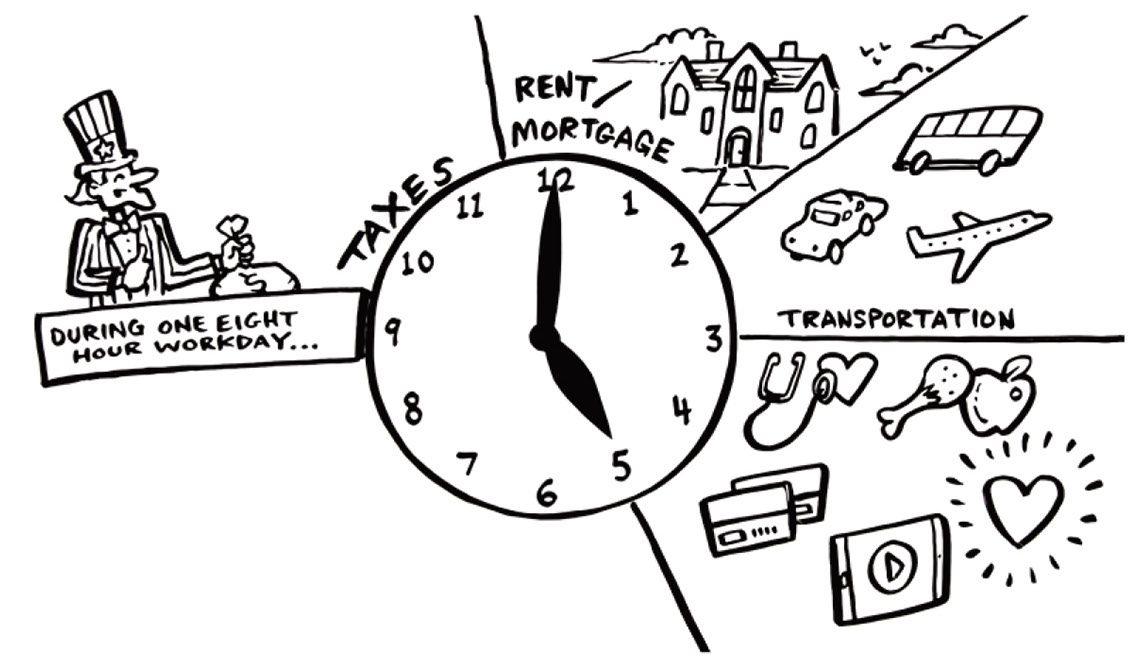
\includegraphics[width=0.9\linewidth,height=0.72\textheight,keepaspectratio]{images/B-59.jpg}
\end{figure}

“嗯，对。”亨利说。“学生贷款。各种东西。当然，还有零碎杂物……”

“餐点，大多时候都是外食。”柔伊说。

“喔，”他朝柔伊手上的拿铁示意，说：“还有咖啡。”

“是的。”她说：“我们可别忘了咖啡。”

“就在这一块。”他说：“原本可以存起来的，你还要挖走几分钟。尽管大部分的人不会这样。所以，一天上班下来，就没有余钱买你想买的照片了。”

尽管听起来很悲哀，最后这几句话却让柔伊非常触动。你想买的照片。她点点头，想听下去，亨利接着要说什么。

“好了。我说过三个秘密，对不对？现在听好，第一个。”

他翻了一页纸，迅速写下一个标题：

{\kaishu 1.先付钱给自己}

“先付钱给自己，”柔伊重复了一遍，自顾着点头说：“那是当然的。”

“你之前听过此一说？”亨利问。

“我不太记得在哪里听说的，但是这话好熟。”

“很好。”亨利说：“你知道这话的意思吗？”

柔伊正想开口说当然知道，但是话到嘴边，却停住了。“我想，我是知道意思的。”

亨利笑着，扬起眉毛，仿佛在问：确定？

“确定，”柔伊说：“当我拿到薪水时，我第一应该把钱花在自己身上。”她看着亨利问：“不是吗？”

亨利笑了笑，“很接近。这是大多数人以为的意思：赚到钱时，第一该犒赏的是自己：买一些好东西、买一点想要的东西。”

“可是，难道不是吗？”

“其实不是，”亨利说：“先付给自己的意思是把钱留给自己，存起来的意思。用另一种方式来说，\textbf{为自己存下第一个小时的收入}。”

亨利翻开新的一页，在上头画图。

\begin{figure}[htbp]
    \centering
    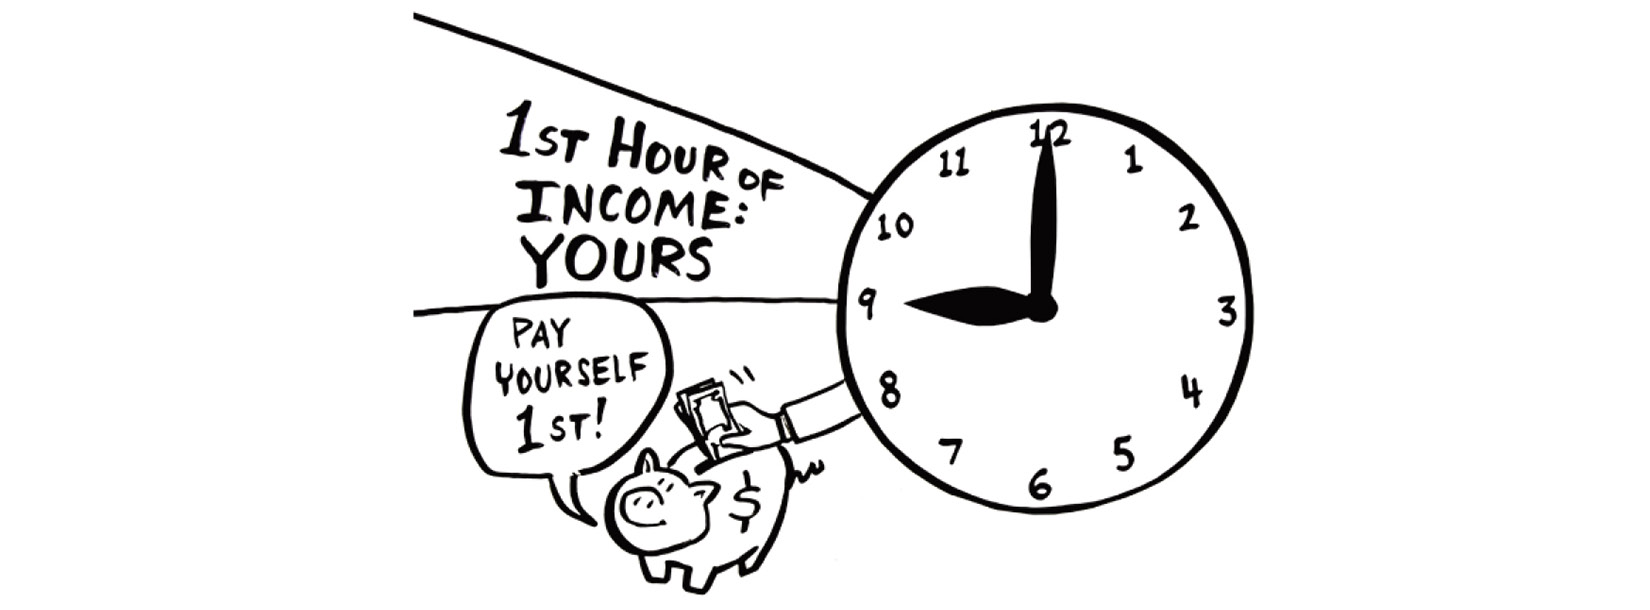
\includegraphics[width=0.9\linewidth,height=0.72\textheight,keepaspectratio]{images/B-61.jpg}
\end{figure}

“去上班是用时间换取金钱。为什么整天工作，而且从周一到周五，”他一边说一边画：“不能至少有1个小时是为了自己做的？虽然大多数人的做法是，拿到薪水后，等政府拿走一大块之后，他们再用剩下的钱去付帐单、买东西。如果这之后，还有钱多下来，而且不是一个小零头，或许他们才有可能为自己存起来。换一种方式来说，就是他们先付了其他人，最后才留给自己。如果还有结余。

“这就是为什么大多数人每天工作8、9、10个小时，日复一日，年复一年，一辈子大约工作9万个小时，9万个小时啊！最后退休之后，却发现帐户里没什么结余。因为他们的钱都用去帮助别人累积财富，却没有帮到自己。”

柔伊沉默一会儿。她的父母不就是这样的吗？

“哇！”她说。

“是啊！哇！”亨利同意。

一阵短暂的沉默之后，柔伊说：“那么，该如何做到？”

亨利认真的看了柔伊一眼，说：“在你还是小女孩时，有没有把零钱丢进存钱筒里？存一段时间，去买一样想要的礼物。”

柔伊还真的这么做过，虽然已经不是小女孩的时候了，当时她18岁，刚去纽约开始大学生活。那个暑假，她1美元1美元的省，3个月后她买下了一辆自行车，从此她开始探索新城市。这个举动叫她自己都很惊讶，因为她在理财方面一向没什么概念。后来，她也试过，在厨房流理台上放一个罐子，朝里头丢10美元，或20美元，但后来都没用，因为总会有些事发生，然后罐子里的钱就花光了。

“这是同样的道理。”亨利说，“和丢零钱到罐子里一样的，你把零碎的钱先用来‘支付给自己’。也可以说，那是一个退休帐户。”

“就像401（k）帐户\footnote{401k帐号：也称退休福利计划，是美国在1981年创立的一种退休金帐户计划，政府把相关规定都纳入在国税法第401（k）条目中，因此简称为401K计划，个人的退休帐户也称为401k帐号。}。”柔伊说。

柔伊上班的杂志社参加了401（k）计划，她记得刚来上班时，就被告知了这一点。后来，她也一直都会收到邮件通知，不断提醒她有空坐下来，设置好自己的退休帐户。

“其实401（k）的设计构想非常简单，”亨利说：“每次你赚到一笔钱，就有部分会拨过去，比方说10％好了，在政府课税前，就先拨到那个帐户去。日积月累，复利加上去，就很可观了。”

“复利是怎样算的？”柔伊问。在遣词用句方面，柔伊很在行，但是说到数学，她就不行了。

她的疑惑没有逃过亨利的眼睛，他说：“现在，就让我来解释给你听。”他伸手到自己口袋里，掏出一张5元的美钞，放在桌面上他和柔伊中间的地方。

“比方说，你每天把5元放在一个存钱桶里。1周后，存钱桶里会有多少钱？”

“1天5元，1周后吗？”柔伊问，那还不简单。“35元。”

亨利点头。“也就是说1个月会有150元。现在我们假设你每天放5元在一个复利帐户，每年利息是10％。你知道，1年之后，这个帐户会有多少钱吗？”

柔伊想一想，150元乘以12吧？“我不太确定。应该比1,500多一点吧？”

亨利点头。“加入复利之后，应该是1,885元\footnote{这里采按月计息，公式为150×（1＋年利率10％÷12）=151.25，第二个月股计算方式是第二个月存150元再加上第一个月的本息，以此类推。}。让我们再来看一看，更久之后会发生什么事。”

他又从口袋里掏出一个小计算机来，开始在键盘上按数字。现在，还有谁会用这种计算机啊？柔伊想，自顾着笑起来。这位咖啡师还真老套。

亨利停了下来，看着柔伊说：“我们就继续用1天5美元来算，过了40年之后，你觉得该是多少呢？”

“我不知道，可能……”柔伊猜想，该不会是5万吧？但好像应该再多一点才是，于是她就把5万加了1倍。“10万？”

亨利笑着回答：“不，差不多10倍。”他把小本子递给柔伊，上头写着：

\begin{figure}[htbp]
    \centering
    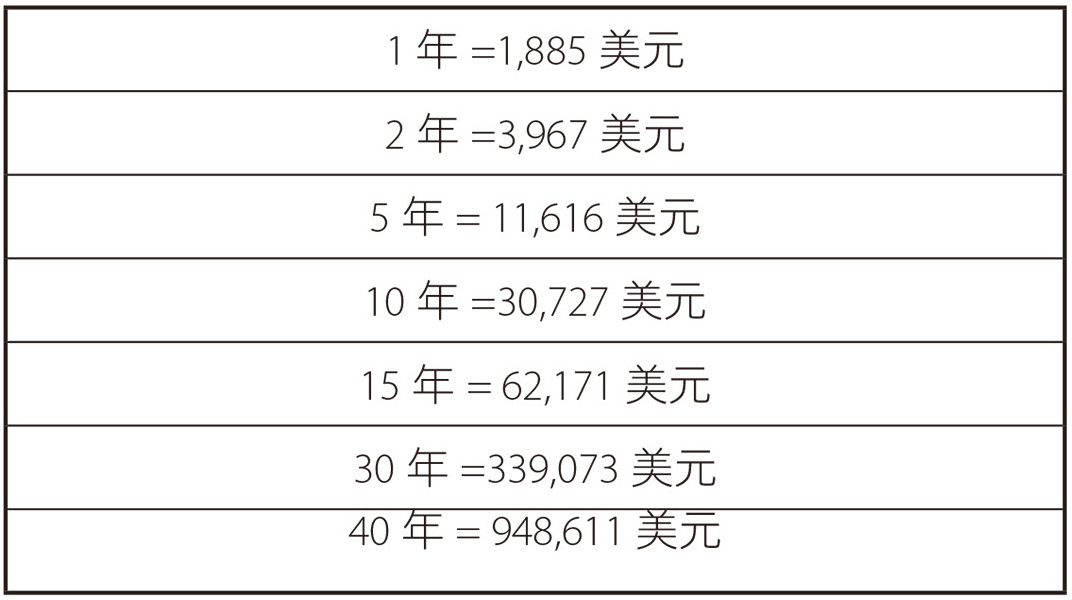
\includegraphics[width=0.6\linewidth]{images/B-65.jpg}
    \caption{一天存5美元，复利10％，40年后能存多少？}
\end{figure}

柔伊看着这一列数字，“可是……”她结巴着问：“可是，真是几乎是100万了耶。”

“没错。是接近100万。”亨利回答。他从口袋里掏了1张10美元的钞票出来，把它放在5美元的上方。

“现在，我们抬高本金，假如我们一天付给自己10美元，放在我们的税前帐户上。我们来算一算40年后的情形”

\begin{figure}[htbp]
    \centering
    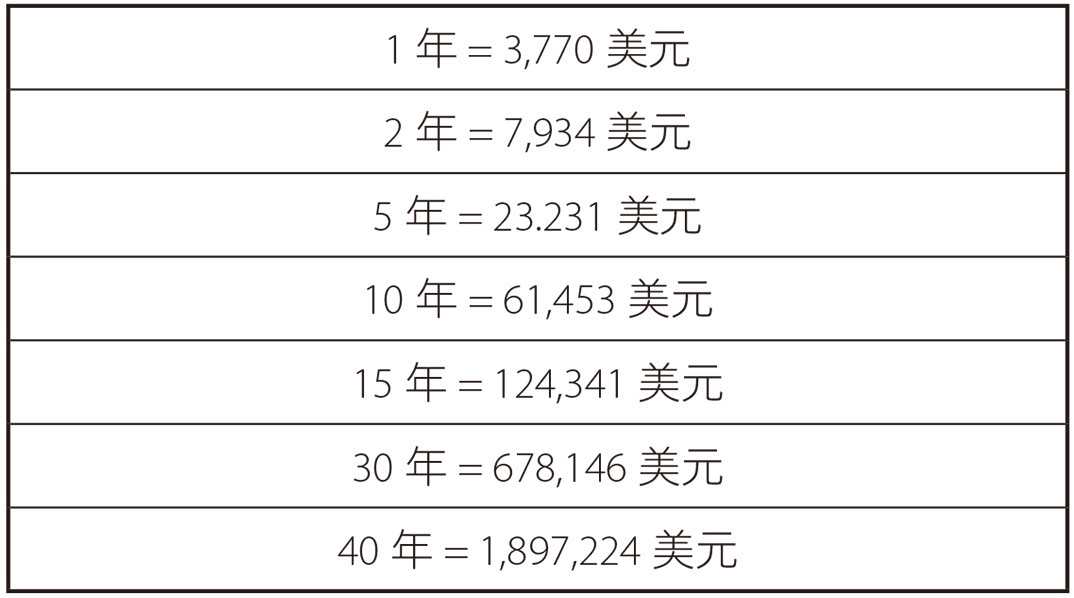
\includegraphics[width=0.6\linewidth]{images/B-66.jpg}
    \caption{同样算法，放进税前账户金额大不同}
\end{figure}

柔伊看着这一列数字，愈往下，眼睛瞪得愈大。“哇！”她说：“你怎么做到的？”

亨利笑着说：“我没有做什么，柔伊。这是大自然做到的。世界就是这样运作的。细菌是如此复倍生长的、谣言也是这样传播的。财富的创建也是如此。也有人说，这是宇宙间最强大的力量，复利的神奇之处也就在于此。”

柔伊看着他手上的试算表。怎么可能呢？

“每天只要10美元……？”柔伊嘀咕着。

“每天只要10美元，”亨利重复了一遍，“但是每天10美元可以改变你的人生。但我要强调一下，以免误解，行为本身是一个小事，丢零钱到存钱桶，每天存10美元，这是一个很小的动作，但是决心做这件事，却不是一个小决定。”他微笑，“这是一个人一辈子最重要的决定。”

柔伊的耳中回响起芭芭拉的声音：那就对了，就做点什么吧！

“现在，让我来再为你举一个例子。”亨利说：“有一个更重要的因素。你今年几岁？”在柔伊回答之前，他又补充说：“我知道一个绅士不该问这样的问题，不过这只是看在科学的分上。而且，我很会保密的。”

“好吧。看在科学的分上，”柔伊一脸正色的说：“27岁。”

“非常棒，”亨利说：“现在，让我们假设你的周薪是1,000美元，你看，我还是很绅士的，没有直接问你薪水。”柔伊笑了起来，事实是，这个数字很接近她实际的周薪。“也就是说，1天200美元。” 亨利继续说：“第一条金律，每天第一个小时的薪水存起来。1天1小时，用另一句话来说，就是先付薪水给你自己。”

“许多人甚至做不到这一点。美国的存款率低于4％，也就是说能存下来的占不到他们收入的4％。若照这个比例，也就是说我们每天只为自己工作20分钟。还有两成的人，完全存不到钱，也就是说，他们付给自己0元。”

“喔！”柔伊嘀咕了一声。那就是她，没错：完全零存款。

“假设你每天工作8小时，”亨利继续说：“让我们把柔伊工作第一个小时赚到的留给柔伊，那就会是……”在计算时，亨利低下头，“1天25美元，或许说1周125元。乘以52周，那么1年就会有6,500元，如果加上年利率4％的复利，就将近6,800元。”

他拿出迷你计算机，开始做另一张试算。

柔伊看着他的计算结果，觉得自己的心跳都加快了。

\begin{figure}[htbp]
    \centering
    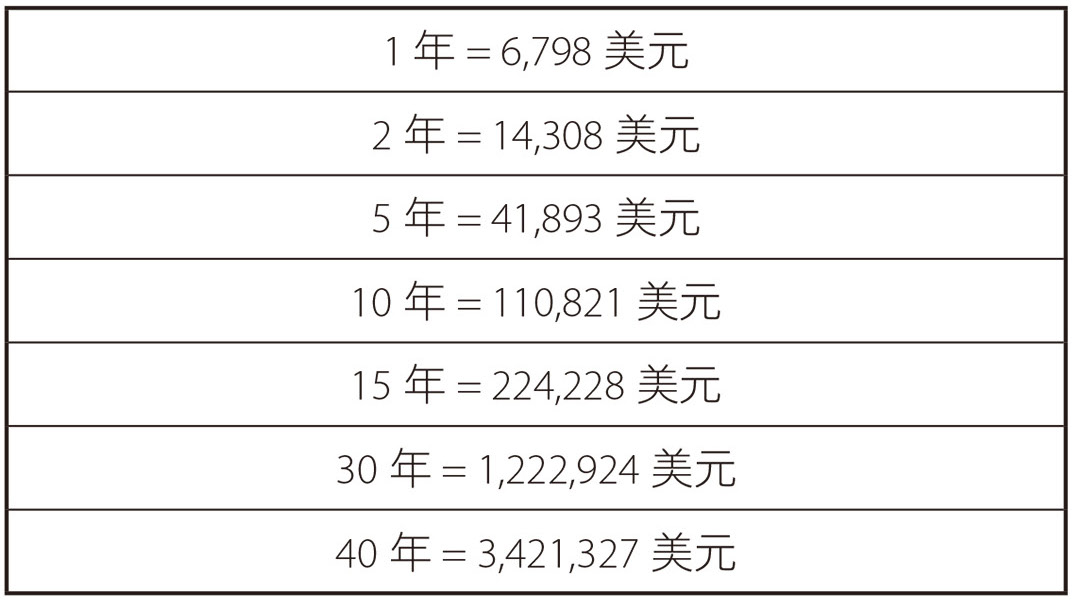
\includegraphics[width=0.6\linewidth]{images/B-69.jpg}
    \caption{1天存25美元，一周存125美元，复利10％，40年后能存多少？}
\end{figure}

\subsection{数字后的意义更重要，应优先考量自己}

亨利写完1个工作放下笔坐回椅子上，等待柔伊看完。

柔伊坐直身体，瞪着数字，300万。只要1天存1个小时的薪水。

亨利瞄了一眼手表，“时间快到了。”他平静的说：“你可能要用跑的。”

柔伊吃了一惊，看了手机一眼，立即跳起来。“我的老天，我真的要走了。”她说。

“走吧！”亨利从高脚椅上滑下来，“我送你到门口。”

他们往咖啡厅大门走过去时，柔伊说：“这个看起来太……我不知道该怎么说，似乎太简单了。”

“是很简单。”亨利回答：“世界就是这样的。往往不是复杂的观念，而是最简单的观念会改变人们的生活。”

“我喜欢你1天10美元的说法。”她说。

他朝着柔伊手中的拿铁点头、微笑：“就是你手上的一杯饮料。你的拿铁因子。”

“没错。”她回答时，他们已经到了咖啡厅的门口。“我的拿铁因子。”此时，她对拿铁因子后面的意义还不甚了解。“这真的很有启发意义。”她临走前伸出手来，和亨利握手。

“啊，对了。”亨利看着她一脸疑惑的样子。温和的说：“柔伊，现在把那些数字都忘了吧！\textbf{数字后面的意义更重要。那就是把你放在一个优先的位置上，先留一些钱给自己}。”

柔伊皱了眉。她忍不住想起了妈妈对她说过的话，先考虑别人，柔伊，永远都要先想一想别人。

亨利肯定的点了点头。“我懂，这和你过去所受的教育不太一样，对不对？好人是不会把自己放在第一位的，总要先为别人着想。你是不是在犹豫这个？”

“差不多。”柔伊坦承。

亨利点头。“那也没错。为别人着想形塑出我们的人类文明。但是人生有时候很吊诡，\textbf{有时候，只有把自己放在第一，才能够服务他人}。这话的意思，你懂吗？”

“坦白说，”柔伊回答：“我不懂。”

“你搭飞机前，有听过起飞前的安全解说吗？里头说到一个，就是遇见问题时，要先把自己的氧气罩戴好，再去帮助你的孩子？听起来好像本末倒置了。你觉得，他们不是应该让乘客先照顾小孩吗？但答案是否定的。因为假如你失去知觉，就不可能再照顾别人的。明白吗？”

“这个我同意。”柔伊说。

亨利把另一只手放在握着柔伊的手上方。“下面是我想说的重点。我相信，我们每个人来到地球上，都有特别的使命。做一些他人无法完成的事。而我们大多数人，却未能完成我们该做的事，只因为我们总是把别人放在第一。”

搭上L线去上班的路上，柔伊想着亨利的话：

{\kaishu 我相信，我们每个人来到地球上，都有特别的使命。而我们大多数人，却未能完成我们该做的事。}

她相信此一说吗？

如果相信，柔伊来这个世上，是该做什么的呢？
